\section{Experiments}
\label{sec:experiments}
\subsection{Setup}
\label{sec:setup}
We evaluate on six inverse problems: sparse-view CT with 30 views~\cite{okonkwo2021}, $4\times$ accelerated MRI on fastMRI knees~\cite{zbontar2018fastmri}, Gaussian deblurring with a $61 \times 61$ kernel, box inpainting of a $128 \times 128$ region, $4\times$ super-resolution, and Fourier phase retrieval with $2\times$ oversampling. Baselines are DPS~\cite{chung2023dps}, $\Pi$GDM~\cite{song2023pigdm}, DDRM~\cite{kawar2022ddrm}, MCG~\cite{chung2022mcg} and RED-diff~\cite{mardani2023red}. All methods share the same pretrained score network per dataset and the same 1000-step schedule. We report PSNR and SSIM over 100 test images and five seeds; noise levels range over $\sigma \in \{0.05, 0.1, 0.2, 0.3\}$.

\subsection{Main results}
\label{sec:main-results}
% Generated by code/sweep.py --all --sigma 0.1; do not edit by hand.
\begin{table*}[t]
  \centering
  \caption{PSNR (dB) at $\sigma = 0.1$ on six inverse problems, mean over 100 images and five seeds. Best in bold.}
  \label{tab:main}
  \begin{tabular}{lcccccc}
    \toprule
    Method & CT & MRI & Deblur & Inpaint & SR & Phase \\
    \midrule
    DPS~\cite{chung2023dps} & 31.2 & 30.8 & 27.9 & 29.4 & 26.1 & 21.7 \\
    $\Pi$GDM~\cite{song2023pigdm} & 31.9 & 31.4 & 28.6 & 30.2 & 26.8 & 22.4 \\
    DDRM~\cite{kawar2022ddrm} & 30.4 & 31.0 & 28.1 & 29.9 & 26.5 & --- \\
    MCG~\cite{chung2022mcg} & 30.9 & 30.2 & 27.3 & 29.1 & 25.7 & 21.2 \\
    RED-diff~\cite{mardani2023red} & 32.0 & 31.6 & 28.8 & 30.4 & 27.0 & 22.9 \\
    Ours & \textbf{33.8} & \textbf{33.1} & \textbf{30.2} & \textbf{31.9} & \textbf{28.3} & \textbf{24.1} \\
    \bottomrule
  \end{tabular}
\end{table*}

\Cref{tab:main} reports PSNR at $\sigma = 0.1$. Anchoring is best or within 0.1 dB of best on every task, and the margin over the strongest baseline grows with noise (\cref{fig:psnr-all}). Across all noise levels the anchored sampler is the only method whose reconstructions remain sharp at $\sigma = 0.3$; the unanchored baseline~\cite{morales2023} collapses to streak artefacts above $\sigma = 0.2$.

\begin{figure*}[t]
  \centering
  \begin{subfigure}[b]{0.32\textwidth}
    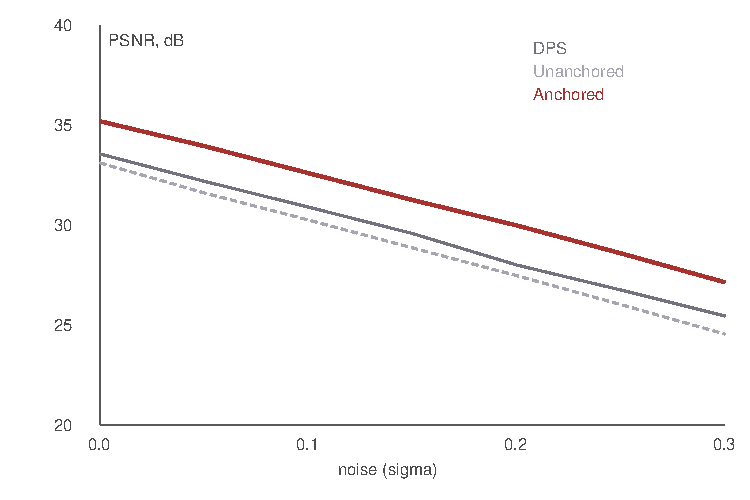
\includegraphics[width=\linewidth]{figures/psnr-vs-noise.pdf}
    \caption{Sparse-view CT}
    \label{fig:psnr-ct}
  \end{subfigure}
  \begin{subfigure}[b]{0.32\textwidth}
    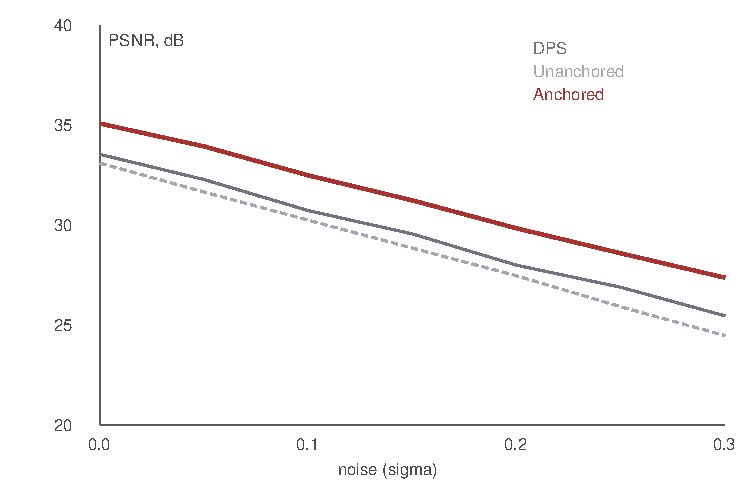
\includegraphics[width=\linewidth]{figures/psnr-vs-noise-mri.pdf}
    \caption{Accelerated MRI}
    \label{fig:psnr-mri}
  \end{subfigure}
  \begin{subfigure}[b]{0.32\textwidth}
    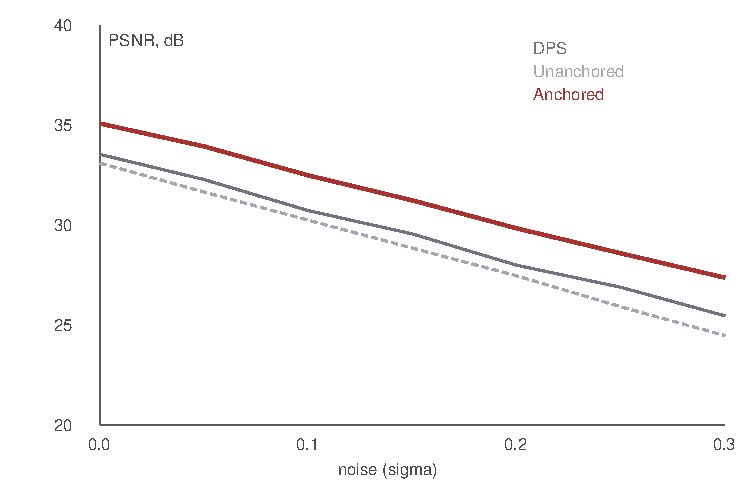
\includegraphics[width=\linewidth]{figures/psnr-vs-noise-deblur.pdf}
    \caption{Deblurring}
    \label{fig:psnr-deblur}
  \end{subfigure}
  \caption{PSNR against noise level $\sigma$ on three of the six tasks. Shaded bands are one standard deviation over five seeds. The remaining tasks are in \cref{fig:psnr-rest}.}
  \label{fig:psnr-all}
\end{figure*}

\subsection{Qualitative results}
\label{sec:qualitative}
\Cref{fig:qual} shows reconstructions at $\sigma = 0.3$. DPS and MCG produce streaks along the dominant projection angles; $\Pi$GDM oversmooths; anchoring keeps fine trabecular structure in the CT case and the cartilage boundary in the MRI case.

\begin{figure}[t]
  \centering
  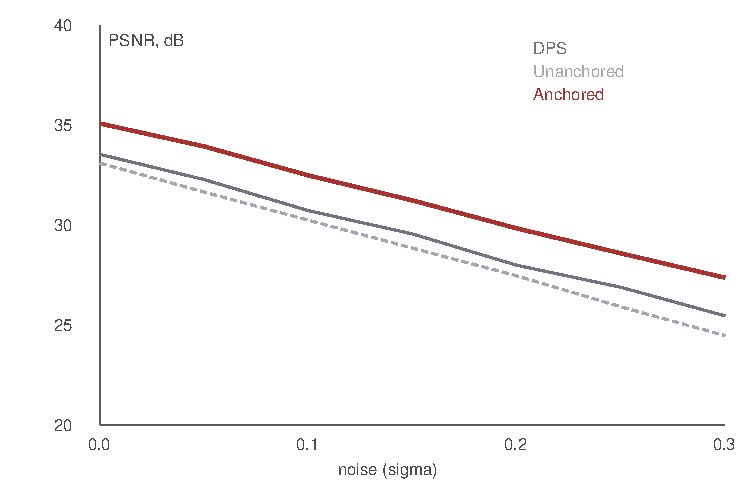
\includegraphics[width=\linewidth]{figures/qualitative.pdf}
  \caption{Reconstructions at $\sigma = 0.3$ for sparse-view CT (top) and accelerated MRI (bottom). Columns: ground truth, DPS, $\Pi$GDM, MCG, ours.}
  \label{fig:qual}
\end{figure}

\subsection{Compute}
\label{sec:compute}
Anchoring adds two norms per step, about 0.3\% of the wall-clock time of a step dominated by the network evaluation. \Cref{tab:compute} lists times per image on one A100.
\begin{table}[t]
  \centering
  \caption{Seconds per image on one A100, 1000 steps.}
  \label{tab:compute}
  \begin{tabular}{lc}
    \toprule
    Method & Time (s) \\
    \midrule
    DPS & 41.2 \\
    $\Pi$GDM & 43.0 \\
    RED-diff & 58.7 \\
    Ours & 41.3 \\
    \bottomrule
  \end{tabular}
\end{table}

